%%%%%%%%%%%%%%%%%%%%%%%%%%%%%%%%%%%%%%%%%
% Beamer Presentation
% LaTeX Template
% Version 1.0 (10/11/12)
%
% This template has been downloaded from:
% http://www.LaTeXTemplates.com
%
% License:
% CC BY-NC-SA 3.0 (http://creativecommons.org/licenses/by-nc-sa/3.0/)
%
%%%%%%%%%%%%%%%%%%%%%%%%%%%%%%%%%%%%%%%%%

%----------------------------------------------------------------------------------------
%	PACKAGES AND THEMES
%----------------------------------------------------------------------------------------

\documentclass[aspectratio=32]{beamer}
\usefonttheme[onlymath]{serif}


\mode<presentation> {

% The Beamer class comes with a number of default slide themes
% which change the colors and layouts of slides. Below this is a list
% of all the themes, uncomment each in turn to see what they look like.

\usetheme{default}
%\usetheme{AnnArbor}
%\usetheme{Antibes}
%\usetheme{Bergen}
%\usetheme{Berkeley}
%\usetheme{Berlin}
%\usetheme{Boadilla}
%\usetheme{CambridgeUS}
%\usetheme{Copenhagen}
%\usetheme{Darmstadt}
%\usetheme{Dresden}
%\usetheme{Frankfurt}
%\usetheme{Goettingen}
%\usetheme{Hannover}
%\usetheme{Ilmenau}
%\usetheme{JuanLesPins}
%\usetheme{Luebeck}
%\usetheme{Malmoe}
%\usetheme{Marburg}
%\usetheme{Montpellier}
%\usetheme{PaloAlto}
%\usetheme{Pittsburgh}
%\usetheme{Rochester}
%\usetheme{Singapore}
%\usetheme{Szeged}
%\usetheme{Warsaw}

% As well as themes, the Beamer class has a number of color themes
% for any slide theme. Uncomment each of these in turn to see how it
% changes the colors of your current slide theme.

%\usecolortheme{albatross}
%\usecolortheme{beaver}
\usecolortheme{spruce}
%\usecolortheme{beetle}
%\usecolortheme{crane}
%\usecolortheme{dolphin}
%\usecolortheme{dove}
%\usecolortheme{fly}
%\usecolortheme{lily}
%\usecolortheme{orchid}
%\usecolortheme{rose}
%\usecolortheme{seagull}
%\usecolortheme{seahorse}
%\usecolortheme{whale}
%\usecolortheme{wolverine}

%\setbeamertemplate{footline} % To remove the footer line in all slides uncomment this line
%\setbeamertemplate{footline}[page number] % To replace the footer line in all slides with a simple slide count uncomment this line

%\setbeamertemplate{navigation symbols}{} % To remove the navigation symbols from the bottom of all slides uncomment this line
}


\usepackage{graphicx} % Allows including images
\usepackage{booktabs} % Allows the use of \toprule, \midrule and \bottomrule in tables
\usepackage{verbatim}
\usepackage{colortbl}

\usepackage{mathtools} 
\usepackage{amssymb}
\usepackage{mathrsfs}
\usepackage{amsmath}
\usepackage{bm}

\usepackage{ragged2e}
\usepackage{etoolbox}
\usepackage{lipsum}

\usepackage{siunitx,booktabs}
\usepackage{pifont}
\usepackage{array}
\usepackage{tabu,booktabs}
\usepackage{tikz,threeparttable}
\usetikzlibrary{arrows,shapes}

\setbeamertemplate{enumerate items}[circle]
\usepackage{tikz}
\usepackage{adjustbox}

\newcommand\mynum[1]{
  \usebeamercolor{enumerate item}
  \tikzset{beameritem/.style={circle,inner sep=0,minimum size=2ex,text=enumerate item.bg,fill=enumerate item.fg,font=\footnotesize}}%
  \tikz[baseline=(n.base)]\node(n)[beameritem]{#1};
}

\newcommand\mynumm[1]{
  \usebeamercolor{enumerate item}
  \tikzset{beameritem/.style={rectangle,inner sep=0,minimum size=2ex,text=enumerate item.bg,fill=enumerate item.fg,font=\footnotesize}}%
  \tikz[baseline=(n.base)]\node(n)[beameritem]{#1};
}
% COLUMN TYPES
\newcolumntype{L}[1]{>{\raggedright\let\newline\\\arraybackslash\hspace{0pt}}m{#1}}
\newcolumntype{C}{>{\centering\arraybackslash}p{5.2em}}
\newcolumntype{D}{>{\centering\arraybackslash}p{5em}}
\newcolumntype{G}{>{\centering\arraybackslash}p{6em}}
\newcolumntype{R}[1]{>{\raggedleft\let\newline\\\arraybackslash\hspace{0pt}}m{#1}}



\def\Put(#1,#2)#3{\leavevmode\makebox(0,0){\put(#1,#2){#3}}}

\setbeamertemplate{footline}[frame number]

\AtBeginSection[]{
  \begin{frame}
  \vfill
  \centering
  \begin{beamercolorbox}[sep=8pt,center,shadow=true,rounded=true]{title}
    \usebeamerfont{title}\insertsectionhead\par%
  \end{beamercolorbox}
  \vfill
  \end{frame}
}

%----------------------------------------------------------------------------------------
%	TITLE PAGE
%----------------------------------------------------------------------------------------

\title{The Welfare Effects of Infrastructure Quality: \\ Evidence from Water Pipe Replacements in Manila} % The short title appears at the bottom of every slide, the full title is only on the title page

\author{\\Will Violette \\ Federal Trade Commission \\ wviolette@ftc.gov \\[2em] Any opinions expressed herein are those of the authors
and do not necessarily represent the views of the
Federal Trade Commission.} 


 % Your institution as it will appear on the bottom of every slide, may be shorthand to save space

\date{November 2020} %\today} % Date, can be changed to a custom date

\begin{document}

\beamertemplatenavigationsymbolsempty

\begin{frame}
\titlepage % Print the title page as the first slide
\end{frame}

%\begin{frame}
%\frametitle{Overview} % Table of contents slide, comment this block out to remove it
%\tableofcontents % Throughout your presentation, if you choose to use \section{} and \subsection{} commands, these will automatically be printed on this slide as an overview of your presentation
%\end{frame}

%----------------------------------------------------------------------------------------
%	PRESENTATION SLIDES
%----------------------------------------------------------------------------------------
%------------------------------------------------

% Mitlin, D., V.A. Beard,
% D. Satterthwaite, and J. Du. 2019. "Unaffordable and
% Undrinkable: Rethinking Urban Water Access in
% the Global South." Working Paper. Washington, DC:
% World Resources Institute. Available online at www.
% citiesforall.org.

\begin{frame}
\frametitle{Replacing Water Pipes}
\centering

% HIGHLIGHT PUBLIC FINANCE

% push punchline at the MOTIVATION!!

\begin{itemize}
  \item 12 out of 15 developing cities have intermittent water supply 
    \begin{itemize}
      \item Most people boil tap water before drinking [WRI, 2019]
    \end{itemize}
  \vspace{2mm}
  \item Fixing water pipes has high fixed costs, but produces marginal cost savings and health benefits
  \vspace{2mm}
\begin{center}

\includegraphics[scale=.5]{tables/nytimespic.png} \\
New York Times, Nov. 10th, 2017
\end{center}
  \vspace{2mm}

  \item Consumer surplus is often absent from the policy dialogue 
  % Policymakers Water quality can affect health (infant mortality, disease)
  %   \vspace{2mm}
  % \item This paper focuses on consumer surplus from water quality

  %%% THIS IS FINE BUT NOT THE KEY REASON!
\end{itemize}
\end{frame}

% https://www.nytimes.com/2017/11/10/climate/water-pipes-plastic-lead.html

% % %------------------------------------------------

\begin{frame}
\frametitle{This paper}
\centering
% In developing countries, 30\% of urban pop live in slums (UN, 2015)

%%% SUBHEADINGS! %%%

% multidimensional water quality at the front

\begin{itemize}
  \item \textbf{Research Question}: how do pipe replacement projects affect welfare?
    \begin{itemize}
      \item Households consume more water 
      \item Households spend less on substitutes for water quality \\
      (filters, storage containers, booster pumps)
      \item Pumping costs decrease and billing increases for the utility
    \end{itemize}
  \vspace{2mm}
  \item \textbf{Method}: analyze the staggered roll-out of 600 km of new pipe in Manila with billing records and survey data on water quality
  \vspace{2mm}
  \item \textbf{Preview of Findings}: pipe replacements lead to 10\% more water consumption and 54\% less booster pump use
    \begin{itemize}
      \item Cost savings alone $<$ Fixed costs
      \item Cost savings + Consumer surplus $>$ Fixed costs
    \end{itemize}
  % \vspace{2mm}
  % \item \textbf{Welfare}: consumer surplus increase equals 40\% of an average water bill
  %   \begin{itemize}
  %     \item 1/3 from better water quality and 2/3 from less spending on booster pumps
  %     \item Consumer surplus + Cost reductions $>$ Fixed costs
  %   \end{itemize}

\end{itemize}

\end{frame}




% % %------------------------------------------------

\begin{frame}
\frametitle{Data on Piped Water in Manila}
\centering

\begin{itemize}
  \item A large, regulated monopoly in Manila provided billing records for 1.5 mil. connections from 2008-2015
  \vspace{3mm}
  \item Billing records merge with survey data on 50,000 total residential connections spread across 2008, 2010, and 2011
    \begin{itemize}
      \item Outcomes measured per household and weighted by household
    \end{itemize}
  \vspace{3mm}
  \item The pipe replacement year is identified for each small-area ($\sim$2,900) according to the year  that accounts for the greatest amount of pipe replacement in each area
    \begin{itemize}
      \item Only consider replacements for areas with pre/post data
      \item Robust to using nearest pipe to each connection
    \end{itemize}
\end{itemize}

% smalla rea size

\end{frame}




% % %------------------------------------------------

\begin{frame}
\frametitle{Water Quality Before/After Pipe Replacement}
\centering

% treatment areas

\begin{table}[h!] 
\centering
% \caption{Average Survey Responses Before and After Pipe Replacement}
\vspace{-2mm}
\begin{threeparttable}
\begin{tabular}{@{}l*{1}{ccc}@{}}
\toprule
  & Before & After  & All \\
\midrule
% Piped Water Service Quality \\[.5em]
$\text{Water has strong pressure (6pm-12am)}^{\dagger}$ & 0.26 & 0.56 & 0.48 \\
$\text{Water has no pressure (6pm-12am)}^{\dagger}$  & 0.29 & 0.04 & 0.09 \\
Water interruptions in last 3 months & 2.28 & 1.93 & 2.13 \\
Water has foreign bodies & 0.23 & 0.05 & 0.14 \\
Water is discolored & 0.08 & 0.03 & 0.04 \\
Water has unusual taste/smell & 0.12 & 0.03 & 0.05 \\
\\[-.5em]
Households & 13,441 & 8,461 & 57,018 \\
\bottomrule
\end{tabular}
\begin{tablenotes}
\footnotesize
\item  $\dagger$ when not using booster pump.\,\,
% See Appendix~\ref{appendix:sampleconstruction} for more details on the sample construction.
\end{tablenotes}
\end{threeparttable}
\end{table}
\begin{itemize}
  \item Large quality improvements
\end{itemize}

\end{frame}
% % \begin{frame}
% % \frametitle{Public Housing in South Africa}
% % % \centering
% % \centering
% % \begin{itemize}
% %   \item Large 
% %     \vspace{2mm}
% %   \item 
% %     \vspace{2mm}
% %   \item 
% % \end{itemize}
% % \end{frame}

% % %------------------------------------------------



\begin{frame}
\frametitle{Quality Substitutes Before/After Pipe Replacement}
\centering

\begin{table}[h!] 
\centering
% \caption{Average Quality Substitutes Before/After Pipe Replacement}
% \vspace{-2mm}
\begin{threeparttable}
\begin{tabular}{@{}l*{1}{ccc}@{}}
\toprule
  & Before & After  & All \\
\midrule
Uses booster pump & 0.37 & 0.11 & 0.16 \\
Hours booster pump is used per day & 2.86 & 2.47 & 2.51 \\
Uses water storage tank & 0.43 & 0.36 & 0.39 \\
Uses water filter & 0.12 & 0.12 & 0.11 \\
Purchases filtered water & 0.68 & 0.74 & 0.69 \\
Purchases from a deepwell & 0.05 & 0.02 & 0.03 \\
Spending on non-piped water (PhP) & 90.93 & 88.26 & 86.99 \\
Drinks from the tap & 0.50 & 0.46 & 0.52 \\
Boils tap water before drinking & 0.23 & 0.19 & 0.21 \\
\\[-.5em]
Households & 13,441 & 8,461 & 57,018 \\
\bottomrule
\end{tabular}
\begin{tablenotes}
\footnotesize
\item 
% See Appendix~\ref{appendix:sampleconstruction} for more details on the sample construction.
\end{tablenotes}
\end{threeparttable}
\end{table}
\begin{itemize}
  \item Much less booster pump use
  \item Small changes in other substitutes
\end{itemize}

\end{frame}

% % %------------------------------------------------


\begin{frame}
\frametitle{Average Usage per Household with Years to Pipe Replacement}
\begin{figure}
\begin{center}
% \caption{Average Consumption per Household with Years to Pipe Replacement}\label{figure:pipecons}
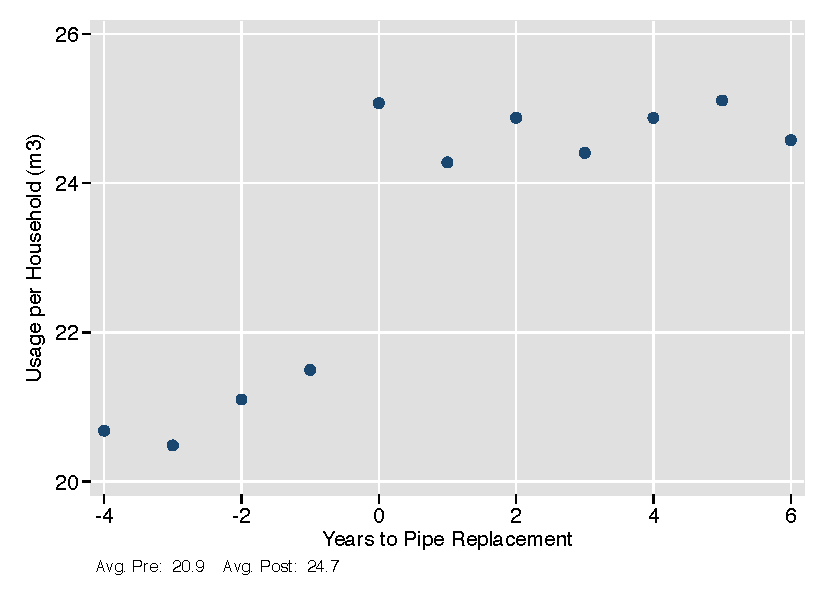
\includegraphics[scale=.73]{tables/pipe_cons.pdf}
\end{center}
%%% add counts and average change in discussion
\end{figure}
\end{frame}

% % %------------------------------------------------



% \begin{frame}
% \frametitle{Price Variation}

% \begin{itemize}
% \item 
%   \begin{itemize}
%   \item Mainly occurs when households start 
%   \end{itemize}
% \item 
% \end{itemize}

% \end{frame}


% % %------------------------------------------------


\begin{frame}
\frametitle{Average Usage per Household with Months to Price Change}
%%% estimate dmeand only for households with a price change

\begin{figure}
\begin{center}
% \caption{Average Consumption per Household with Years to Pipe Replacement}\label{figure:pipecons}
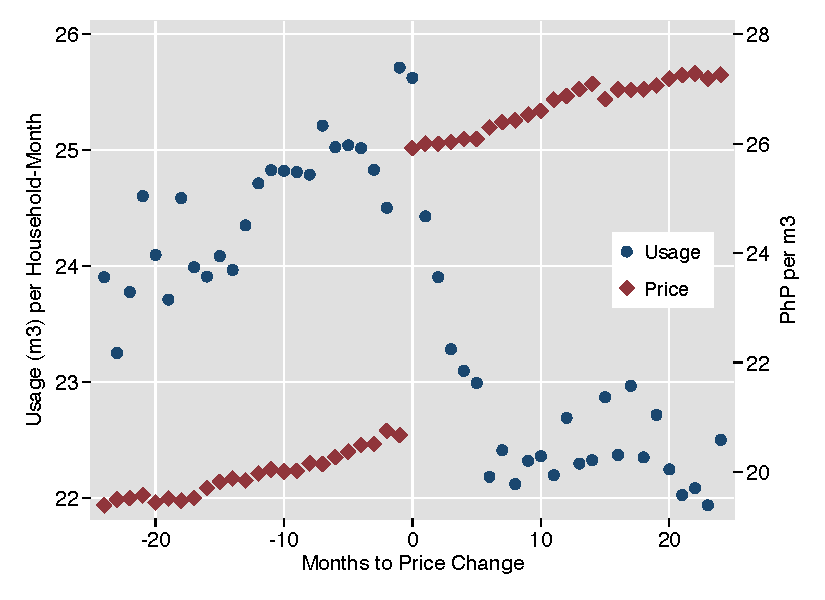
\includegraphics[scale=.54]{tables/r_to_s_only_graph.pdf}
\end{center}
\begin{itemize}
\item 729 households are switched to a high-price tariff when they are detected with businesses (ie. roadside stands)
\item Switched households use more water but have similar demographics to other households
\end{itemize}
%%% add counts and average change in discussion
\end{figure}
\end{frame}


% % %------------------------------------------------


\begin{frame}
\frametitle{Household Demand for Water}

\begin{align*}
\label{eq:utility}
max_{w,x,B} &\hspace{.5cm}\frac{1}{\alpha} \, \Big[ \,  Q(B,R) \,  w  \, -\, \frac{1}{2}(w - \gamma)^2 \, \Big] \, + \, x  \\
s.t.& \\
&p\,w \,+\, x \, +  B \, F \, = Y
\end{align*}

\begin{itemize}
  \item $\alpha$ is the price-sensitivity
  \item $Q(B,R)$ is water quality depending on booster pump use ($B$) and pipe replacements ($R$)
  \item $w$ is water usage
  \item $x$ is all other goods
  \item $\gamma$ is the fixed preference for water
  % \vspace{2mm}
  \item $p$ is the water price (assumed to be constant)
  \item $F$ is the monthly cost of the booster pump
  \item $Y$ is income
\end{itemize}

\end{frame}


\begin{frame}
\frametitle{Solve for the Welfare Effect of Pipe Replacements }

\begin{itemize}
  \item Water demand as a function of booster pump choice
      \begin{align*}
      w \, = \, \gamma \, - \, \alpha p +  Q(B,R)
      \end{align*}
  \item Effect of pipe replacements on consumer welfare
      % \begin{align*}
      % V\,=\,\frac{\alpha p^2}{2} - \gamma p + \frac{Q(B,R)^{2}}{2\alpha} - p Q(B,R) + \frac{\gamma Q(B,R)}{\alpha} + y - B F
      % \end{align*}
      \begin{align*}
      \frac{dV}{dR}\,=\,\frac{w}{\alpha} \frac{dQ}{dR} - F \frac{dB}{dR}
      \end{align*}
\end{itemize}

\end{frame}


\begin{frame}
\frametitle{Estimating Demand}

%%% LINK BACK TO BEFORE, PREVIOUS SHOWING VARIATION

% \begin{itemize}
%   \item Water Demand
% \end{itemize}
\begin{align*}
&\text{First Stage}\\
p_{it} &= \phi_1 \text{Post Pipe}_{tl}  +  \phi_3 \text{Post p ch}_{it} +  \phi_1\text{Pre t}_{it} +\phi_2\text{Post t}_{it} +  \phi_t +  \phi_i + \epsilon_{itl}  \\[.5em]
&\text{Second Stage}\\
w_{itl} &= \gamma_1  \text{Post Pipe}_{tl} + \gamma_2  \hat{p}_{it} + \gamma_3\text{Pre t}_{it} +\gamma_4\text{Post t}_{it} +    \gamma_t +  \gamma_i +  \varepsilon_{itl} \\
b_{itl} &= \beta_1  \text{Post Pipe}_{tl} + \beta_2  \hat{p}_{it} + \beta_3\text{Pre t}_{it} +\beta_4\text{Post t}_{it} +    \beta_t +  \beta_i +  \varepsilon_{itl} 
\end{align*}
\begin{itemize}
  \item $w_{itl}$ is water consumption and $b_{itl}$ is booster pump use
  \item $i$ is household, $t$ is month, and $l$ is location
  \item $\text{Post Pipe}_{tl}$ indicates months after pipe replacements
  \item $\text{Pre t}_{it}$ and $\text{Post t}_{it}$ are pre and post trends relative to the first price change
  \item $\text{Post p ch}_{it}$ indicates months after the first price change
\end{itemize}

\end{frame}

\begin{frame}
\frametitle{Estimating Water Demand}
Second stage
  \begin{align*}
  w_{itl} &= \gamma_1  \text{Post Pipe}_{tl} + \gamma_2  \hat{p}_{it} + \gamma_3\text{Pre t}_{it} +\gamma_4\text{Post t}_{it} +    \gamma_t +  \gamma_i +  \varepsilon_{itl} \\
  b_{itl} &= \beta_1  \text{Post Pipe}_{tl} + \beta_2  \hat{p}_{it} + \beta_3\text{Pre t}_{it} +\beta_4\text{Post t}_{it} +    \beta_t +  \beta_i +  \varepsilon_{itl} 
  \end{align*}
Effect of pipe replacements on consumer welfare
  \begin{align*}
  \frac{dV}{dR}\,=\,\frac{w}{\alpha} \frac{dQ}{dR} - F \frac{dB}{dR}
  \end{align*}

\begin{itemize}
  \item $\gamma_1 = \frac{dQ}{dR} $
  \item $\beta_1  = \frac{dB}{dR}$
  \item $\gamma_2 = \alpha +  \frac{dQ}{dB} \frac{dB}{dp}$
  \item $\beta_2 = \frac{dB}{dp}$
\end{itemize}

\end{frame}




\begin{frame}
\frametitle{Results}

\begin{table}[h!] 
\centering
% \caption{Household Water and Booster Pump Use Estimates}\label{table:mainregs}
\vspace{-2mm}
\begin{threeparttable}
\begin{tabular}{@{}l*{1}{CC}@{}}
\toprule
  % & (1)       &  (2)              \\
  & Water Use & Booster Pump Use \\
\midrule
After Pipe Replacement&        1.88***&       -0.20***\\
                    &      (0.13)   &      (0.03)   \\[0.5em]
Avg. Price (PhP)    &       -0.59***&        0.01   \\
                    &      (0.10)   &      (0.02)   \\[0.5em]
Mean                &       19.83   &        0.16   \\
$\text{R}^{2}$      &       0.002   &       0.043   \\
N                   &   4,004,445   &      10,560   \\
Dataset             &Billing Panel   &Household Survey   \\

\bottomrule
\end{tabular}
\begin{tablenotes}
\footnotesize
\item Includes connection and calendar month fixed effects.  Standard errors are clustered at the small-area level.
\end{tablenotes}
\end{threeparttable}
\end{table}

%%% CALCULATE ELASTICITY

\end{frame}



\begin{frame}
\frametitle{Heterogeneous Effects}

\begin{table}[h!] 
\centering
% \caption{Household Water and Booster Pump Use Estimates}\label{table:mainregs}
% \vspace{-2mm}
    \begin{adjustbox}{width=\textwidth, totalheight=\textheight-2\baselineskip,keepaspectratio}
\begin{threeparttable}
\begin{tabular}{@{}l*{1}{CC}@{}}
\toprule
  % & (1)       &  (2)              \\
  & Water Use &  Booster Pump Use  \\
\midrule
Post                &        1.17***&       -0.22***\\
                    &      (0.33)   &      (0.03)   \\
Post $\times$ Household Size&        0.08   &       -0.00   \\
                    &      (0.06)   &      (0.00)   \\
Post $\times$ Employed Household Members&       -0.12   &        0.01   \\
                    &      (0.10)   &      (0.00)   \\
Post $\times$ High Skilled Employment&       -1.32***&       -0.01   \\
                    &      (0.36)   &      (0.02)   \\
Post $\times$ Subdivided House/Duplex&        0.76*  &       -0.00   \\
                    &      (0.31)   &      (0.01)   \\
Post $\times$ Freestanding House&        1.11***&       -0.01   \\
                    &      (0.28)   &      (0.01)   \\
Mean                &       19.83   &        0.16   \\
Household FE        &  \checkmark   &               \\
Small Area FE       &               &  \checkmark   \\
$\text{R}^{2}$      &       0.006   &       0.026   \\
N                   &   4,004,445   &      48,982   \\
Dataset             &Billing Panel   &Household Survey   \\

\bottomrule
\end{tabular}
\begin{tablenotes}
\footnotesize
\item
% \item Includes connection and calendar month fixed effects.  Standard errors are clustered at the small-area level.
\end{tablenotes}
\end{threeparttable}
    \end{adjustbox}
\end{table}

\end{frame}



\begin{frame}
\frametitle{Effects on Consumer Welfare}

\begin{table}[h!] 
\centering
% \caption{Change in Consumer Surplus}\label{table:mainregs}
\vspace{-2mm}
\begin{threeparttable}
\begin{tabular}{@{}l*{1}{CCC}@{}}
\toprule
            & Better Water Quality              &  Less Spending on Booster Pumps & Total             \\
\midrule
Expression  & $\frac{w}{\alpha} \frac{dQ}{dR}$ &   $- F \frac{dB}{dR}$  & $\frac{dV}{dR}$ \\[1em]
Estimates (in PhP)   &   249.7 & 97.1 & 346.8 \\
            &  (109.6) & (16.8) & (103.7)  \\
% Evaluated Estimates \\
\bottomrule
\end{tabular}
\begin{tablenotes}
\footnotesize
\item 
% Weighting, discussion of different samples, clustering, controls (especially rate classes).  This table predicts usage per household with pipe replacement and price with different fixed effects.  
\end{tablenotes}
\end{threeparttable}

\begin{itemize}
  \item Average water bill per household is 532 PhP
  \vspace{.5mm}
  \item Average monthly household income is 26,023PhP
    \vspace{.5mm}
  \item The monthly operating cost of booster pumps, $F$, is 486 PhP
    \vspace{.5mm}
  \begin{itemize}
    \item Electricity is expensive and pumps are used for 2.6 hrs per day
    \item Does not include upfront price ranging from 1,200 to 15,000 PhP
  \end{itemize}
\end{itemize}

\end{table}

\end{frame}

% %------------------------------------------------

\begin{frame}
\frametitle{Do pipe replacements pay for themselves?}

\begin{table}[h!] 
\centering
% \caption{Total Water Supplied and Billed Estimates}\label{table:nrwregs}
% \vspace{-2mm}
\begin{threeparttable}
\begin{tabular}{@{}l*{1}{CCCCC}@{}}
\toprule
  % & (1)   & (2)   & (3) \\
  & Billing  & Supply Costs \\
\midrule
After Pipe Replacement&       57.07***&      -74.04** \\
                    &      (4.30)   &     (22.77)   \\
Mean                &      531.94   &       27.53   \\
$\text{R}^{2}$      &       0.511   &       0.798   \\
N                   &   4,002,952   &      67,827   \\

\bottomrule
\end{tabular}
\begin{tablenotes}
\footnotesize
\item 
% Say it includes both fixed effects (Describe fixed effects...) .  Weighting, discussion of different samples, clustering, controls (especially rate classes).  This table predicts usage per household with pipe replacement and price with different fixed effects.   \regtext 45 PhP = 1 USD \,\,
\end{tablenotes}
\end{threeparttable}
\end{table}

\begin{itemize}
  \item Fixed costs equal 17,021 PhP per household
  \item 10 year loan at 5\% interest implies monthly payments of 181 PhP
  \item Consumer surplus of 161 PhP + Cost savings of 131 PhP $>$ Loan payments of 181 PhP
  \item Does not include health benefits, commercial users (6\%), other infrastructure benefits
\end{itemize}

\end{frame}


\begin{frame}

\frametitle{Takeaways}

\begin{itemize}
  \item Consumer surplus matters for pipe replacement policies
  \item Important to measure both direct effects (ie. consumption) and indirect effects (ie. quality substitutes) of quality investments
  \item Thanks for coming and for your feedback!
\end{itemize}


\end{frame}


% Section Welfare:
%   - Welfare benefits with 10 yr 5\% loans (assume discount rates) or 50 yr 5\% loan?
%   - Welfare benefits with cash
%   - Are households willing to pay for pipe improvements?

%   - How do welfare estimates compare to traditional estimates from health measures?



\end{document} 
